\documentclass[aspectratio=169,11pt]{beamer}
% =====================================================================
%  pds-beamer.tex — Estilo común de las transparencias.
%
%  Uso (desde teoría/Tx/transparencias/):
%     \documentclass[aspectratio=169,11pt]{beamer}
%     % =====================================================================
%  pds-beamer.tex — Estilo común de las transparencias.
%
%  Uso (desde teoría/Tx/transparencias/):
%     \documentclass[aspectratio=169,11pt]{beamer}
%     % =====================================================================
%  pds-beamer.tex — Estilo común de las transparencias.
%
%  Uso (desde teoría/Tx/transparencias/):
%     \documentclass[aspectratio=169,11pt]{beamer}
%     \input{../../comun/pds-beamer}
%     \title{...}  \subtitle{Tema x · ...}
%     \begin{document}
%       \portada
%       ...
%     \end{document}
%  Compilar con:  latexmk -xelatex  (o «make» desde teoría/)
% =====================================================================

\usetheme{Boadilla}
\usecolortheme{orchid}
\usefonttheme{professionalfonts}
\setbeamercovered{transparent}
\setbeamersize{text margin left=0.8cm, text margin right=0.8cm}
\setbeamertemplate{navigation symbols}{}
\setbeamertemplate{itemize item}[square]
\setbeamertemplate{itemize subitem}[circle]
\setbeamertemplate{itemize subsubitem}[triangle]
\setbeamertemplate{enumerate item}[square]
\setbeamertemplate{enumerate subitem}[circle]
\setbeamertemplate{caption}{\raggedright\insertcaption\par}

\input{../../comun/pds-comun.tex}

% Tipografía: Fira Sans + Fira Math (legibles en proyector)
\usepackage{fontspec}
\usepackage{unicode-math}
% Se cargan por nombre de fichero para que funcionen con cualquier
% instalación de TeX Live (o MiKTeX) sin instalar fuentes en el sistema.
\setmainfont{FiraSans}[Extension=.otf, UprightFont=*-Regular, BoldFont=*-SemiBold,
  ItalicFont=*-Italic, BoldItalicFont=*-SemiBoldItalic]
\setsansfont{FiraSans}[Extension=.otf, UprightFont=*-Regular, BoldFont=*-SemiBold,
  ItalicFont=*-Italic, BoldItalicFont=*-SemiBoldItalic]
\setmonofont{FiraMono}[Extension=.otf, UprightFont=*-Regular, BoldFont=*-Medium, AutoFakeSlant=0.15, Scale=0.92]
\setmathfont{FiraMath-Regular.otf}
\setmathfont{latinmodern-math.otf}[range={"229B,"22EE,"22F1}]

% Colores del tema ajustados a la paleta común (más contraste)
\setbeamercolor{structure}{fg=pdsazul}
\setbeamercolor{alerted text}{fg=pdsrojo}
\setbeamercolor{example text}{fg=pdsverde}
\setbeamercolor{block title}{bg=pdsazul, fg=white}
\setbeamercolor{block body}{bg=pdsfondo}
\setbeamercolor{block title alerted}{bg=pdsrojo, fg=white}
\setbeamercolor{block body alerted}{bg=pdsrojo!6}
\setbeamercolor{block title example}{bg=pdsverde, fg=white}
\setbeamercolor{block body example}{bg=pdsverde!6}
\setbeamercolor{frametitle}{fg=pdsazul, bg=white}
\setbeamerfont{frametitle}{size=\large, series=\bfseries}
\setbeamerfont{block title}{size=\normalsize, series=\bfseries}
\setbeamertemplate{blocks}[rounded][shadow=false]

% Logo en la esquina superior derecha de cada transparencia
\pgfdeclareimage[height=0.8cm]{logo}{../../comun/ucm.png}
\addtobeamertemplate{frametitle}{}{%
  \begin{tikzpicture}[remember picture, overlay]
    \node[anchor=north east, inner sep=0pt] at ([xshift=-0.25cm, yshift=-0.2cm]current page.north east) {\pgfuseimage{logo}};
  \end{tikzpicture}}

% Datos de portada
\author[\autorescorto]{\autores}
\institute[UCM]{\footnotesize\departamento\\\universidad}
\date[\curso]{\footnotesize\grado\\\curso}

\newcommand{\portada}{%
  \begin{frame}[plain]
    \begin{center}
      
\includegraphics[height=1.9cm]{../../comun/ucm.png}
    \end{center}
    \vspace{-0.4cm}
    \titlepage
  \end{frame}}

% Índice al empezar cada sección
\AtBeginSection[]{%
  \begin{frame}{Contenido}
    \tableofcontents[currentsection, hideothersubsections]
  \end{frame}}

\renewcommand{\pdscodesize}{\scriptsize}

% Utilidades
% \herramienta{T1-convolucion-continua}: enlace a la página publicada de
% herramientas/html (se abre en el navegador, sin instalar nada).
% \herramientaservidor{server/....py}: app que necesita Python (bokeh serve).
\newcommand{\urlherramientas}{https://ucm-237.github.io/PdS/}
\newcommand{\herramienta}[1]{%
  \par\vfill\hfill{\scriptsize\color{pdsgris}\faIcon\ \href{\urlherramientas#1.html}{Herramienta interactiva: \texttt{#1}}}}
\newcommand{\herramientaservidor}[1]{%
  \par\vfill\hfill{\scriptsize\color{pdsgris}\faIcon\ Herramienta interactiva (con Python): \texttt{herramientas/#1}}}
\newcommand{\faIcon}{\textbf{▶}}
\newcommand{\gris}[1]{{\color{pdsgris}#1}}
\newcommand{\nota}[1]{\par\vspace{2pt}{\footnotesize\color{pdsgris}\textit{#1}}\par}
% Nota sobre una errata de versiones anteriores (solo con \ERRATAS)
\newcommand{\errata}[1]{\iferratas\nota{Errata de versiones anteriores: #1}\fi}
\newcommand{\apuntes}[1]{\nota{Más detalle en los apuntes, #1.}}

% Bloques con nombre en castellano
\newenvironment{definicion}[1][Definición]{\begin{block}{#1}}{\end{block}}
\newenvironment{importante}[1][Importante]{\begin{alertblock}{#1}}{\end{alertblock}}
\newenvironment{ejemplo}[1][Ejemplo]{\begin{exampleblock}{#1}}{\end{exampleblock}}

%     \title{...}  \subtitle{Tema x · ...}
%     \begin{document}
%       \portada
%       ...
%     \end{document}
%  Compilar con:  latexmk -xelatex  (o «make» desde teoría/)
% =====================================================================

\usetheme{Boadilla}
\usecolortheme{orchid}
\usefonttheme{professionalfonts}
\setbeamercovered{transparent}
\setbeamersize{text margin left=0.8cm, text margin right=0.8cm}
\setbeamertemplate{navigation symbols}{}
\setbeamertemplate{itemize item}[square]
\setbeamertemplate{itemize subitem}[circle]
\setbeamertemplate{itemize subsubitem}[triangle]
\setbeamertemplate{enumerate item}[square]
\setbeamertemplate{enumerate subitem}[circle]
\setbeamertemplate{caption}{\raggedright\insertcaption\par}

% =====================================================================
%  pds-comun.tex — Paquetes, colores y estilos de código comunes a
%  transparencias, apuntes y hojas de ejercicios. Compilar con XeLaTeX.
%  No cargar directamente: lo cargan pds-beamer.tex y pds-apuntes.tex.
% =====================================================================

\usepackage{polyglossia}
\setmainlanguage{spanish}
\usepackage{mathtools}
\usepackage{graphicx}
\usepackage{booktabs}
\usepackage{multirow}
\usepackage{array}
\usepackage{xcolor}
\usepackage{tikz}
\usetikzlibrary{positioning,arrows.meta,calc,shapes.geometric,decorations.pathreplacing}
\usepackage{listings}
\usepackage{siunitx}
\sisetup{output-decimal-marker={,}, group-separator={\,}, per-mode=symbol}

% Notas de erratas de versiones anteriores: no se imprimen salvo que se
% defina \ERRATAS antes de cargar el estilo (make ERRATAS=1)
\newif\iferratas
\ifdefined\ERRATAS \erratastrue \fi

% Ruta común (logo y figuras compartidas)
\providecommand{\rutacomun}{../../comun/}
\input{\rutacomun datos.tex}

% ---------------------------------------------------------------------
%  Paleta (la misma que usan las figuras generadas con Python,
%  ver comun/pds_estilo.py)
% ---------------------------------------------------------------------
\definecolor{pdsazul}{HTML}{2B3A8C}
\definecolor{pdsrojo}{HTML}{C0392B}
\definecolor{pdsverde}{HTML}{1E7B4F}
\definecolor{pdsnaranja}{HTML}{D9822B}
\definecolor{pdsgris}{HTML}{5A5A66}
\definecolor{pdsfondo}{HTML}{F3F4FA}
\definecolor{pdscodigo}{HTML}{F7F7F2}

% ---------------------------------------------------------------------
%  Diagramas de bloques (TikZ)
% ---------------------------------------------------------------------
\tikzset{
  bloque/.style={rectangle, rounded corners=2pt, draw=pdsazul!80, fill=pdsfondo,
                 very thick, minimum height=8mm, minimum width=14mm, align=center},
  sumador/.style={circle, draw=pdsazul!80, fill=pdsfondo, thick, inner sep=1.5pt},
  flecha/.style={-{Stealth[length=2.2mm]}, thick, pdsgris},
}

% ---------------------------------------------------------------------
%  Código: Python y Matlab en paralelo
% ---------------------------------------------------------------------
\newcommand{\pdscodesize}{\footnotesize}
\lstdefinestyle{pds}{
  basicstyle=\ttfamily\pdscodesize,
  keywordstyle=\color{pdsazul}\bfseries,
  commentstyle=\color{pdsverde}\itshape,
  stringstyle=\color{pdsrojo},
  numbers=none,
  backgroundcolor=\color{pdscodigo},
  frame=single, rulecolor=\color{pdsgris!40}, framerule=0.4pt,
  xleftmargin=2pt, xrightmargin=2pt, aboveskip=2pt, belowskip=2pt,
  columns=fullflexible, keepspaces=true,
  showstringspaces=false, breaklines=true, tabsize=4,
  upquote=true,
  % Con XeLaTeX, listings desordena los caracteres no ASCII junto a
  % dígitos («2π» sale «π2»): se sustituyen por su versión matemática.
  literate={π}{{$\pi$}}1 {δ}{{$\delta$}}1 {ω}{{$\omega$}}1 {Ω}{{$\Omega$}}1
           {≈}{{$\approx$}}1 {µ}{{$\mu$}}1 {·}{{$\cdot$}}1 {α}{{$\alpha$}}1
           {á}{{á}}1 {é}{{é}}1 {í}{{í}}1 {ó}{{ó}}1 {ú}{{ú}}1 {ñ}{{ñ}}1 {¿}{{¿}}1,
}
\lstdefinestyle{python}{style=pds, language=Python,
  morekeywords={as,True,False,None}}
\lstdefinestyle{matlab}{style=pds, language=Matlab,
  morekeywords={function,end,true,false}}

% \codigo{<ruta sin extensión>} muestra el mismo ejemplo en Python
% y en Matlab, uno al lado del otro. Los ficheros viven en
% ../codigo/python/<nombre>.py y ../codigo/matlab/<nombre>.m y se
% ejecutan en las pruebas (make prueba-codigo).
\newcommand{\rutacodigo}{../codigo/}
\newcommand{\codigoetiqueta}[1]{{\sffamily\scriptsize\bfseries\color{pdsgris}#1}}
\newcommand{\codigo}[2][]{%
  \par\noindent
  \begin{minipage}[t]{0.495\linewidth}
    \codigoetiqueta{Python}\par\vspace{1pt}
    \lstinputlisting[style=python,#1]{\rutacodigo python/#2.py}
  \end{minipage}\hfill
  \begin{minipage}[t]{0.495\linewidth}
    \codigoetiqueta{Matlab}\par\vspace{1pt}
    \lstinputlisting[style=matlab,#1]{\rutacodigo matlab/#2.m}
  \end{minipage}\par}

\input{\rutacomun notacion.tex}


% Tipografía: Fira Sans + Fira Math (legibles en proyector)
\usepackage{fontspec}
\usepackage{unicode-math}
% Se cargan por nombre de fichero para que funcionen con cualquier
% instalación de TeX Live (o MiKTeX) sin instalar fuentes en el sistema.
\setmainfont{FiraSans}[Extension=.otf, UprightFont=*-Regular, BoldFont=*-SemiBold,
  ItalicFont=*-Italic, BoldItalicFont=*-SemiBoldItalic]
\setsansfont{FiraSans}[Extension=.otf, UprightFont=*-Regular, BoldFont=*-SemiBold,
  ItalicFont=*-Italic, BoldItalicFont=*-SemiBoldItalic]
\setmonofont{FiraMono}[Extension=.otf, UprightFont=*-Regular, BoldFont=*-Medium, AutoFakeSlant=0.15, Scale=0.92]
\setmathfont{FiraMath-Regular.otf}
\setmathfont{latinmodern-math.otf}[range={"229B,"22EE,"22F1}]

% Colores del tema ajustados a la paleta común (más contraste)
\setbeamercolor{structure}{fg=pdsazul}
\setbeamercolor{alerted text}{fg=pdsrojo}
\setbeamercolor{example text}{fg=pdsverde}
\setbeamercolor{block title}{bg=pdsazul, fg=white}
\setbeamercolor{block body}{bg=pdsfondo}
\setbeamercolor{block title alerted}{bg=pdsrojo, fg=white}
\setbeamercolor{block body alerted}{bg=pdsrojo!6}
\setbeamercolor{block title example}{bg=pdsverde, fg=white}
\setbeamercolor{block body example}{bg=pdsverde!6}
\setbeamercolor{frametitle}{fg=pdsazul, bg=white}
\setbeamerfont{frametitle}{size=\large, series=\bfseries}
\setbeamerfont{block title}{size=\normalsize, series=\bfseries}
\setbeamertemplate{blocks}[rounded][shadow=false]

% Logo en la esquina superior derecha de cada transparencia
\pgfdeclareimage[height=0.8cm]{logo}{../../comun/ucm.png}
\addtobeamertemplate{frametitle}{}{%
  \begin{tikzpicture}[remember picture, overlay]
    \node[anchor=north east, inner sep=0pt] at ([xshift=-0.25cm, yshift=-0.2cm]current page.north east) {\pgfuseimage{logo}};
  \end{tikzpicture}}

% Datos de portada
\author[\autorescorto]{\autores}
\institute[UCM]{\footnotesize\departamento\\\universidad}
\date[\curso]{\footnotesize\grado\\\curso}

\newcommand{\portada}{%
  \begin{frame}[plain]
    \begin{center}
      
\includegraphics[height=1.9cm]{../../comun/ucm.png}
    \end{center}
    \vspace{-0.4cm}
    \titlepage
  \end{frame}}

% Índice al empezar cada sección
\AtBeginSection[]{%
  \begin{frame}{Contenido}
    \tableofcontents[currentsection, hideothersubsections]
  \end{frame}}

\renewcommand{\pdscodesize}{\scriptsize}

% Utilidades
% \herramienta{T1-convolucion-continua}: enlace a la página publicada de
% herramientas/html (se abre en el navegador, sin instalar nada).
% \herramientaservidor{server/....py}: app que necesita Python (bokeh serve).
\newcommand{\urlherramientas}{https://ucm-237.github.io/PdS/}
\newcommand{\herramienta}[1]{%
  \par\vfill\hfill{\scriptsize\color{pdsgris}\faIcon\ \href{\urlherramientas#1.html}{Herramienta interactiva: \texttt{#1}}}}
\newcommand{\herramientaservidor}[1]{%
  \par\vfill\hfill{\scriptsize\color{pdsgris}\faIcon\ Herramienta interactiva (con Python): \texttt{herramientas/#1}}}
\newcommand{\faIcon}{\textbf{▶}}
\newcommand{\gris}[1]{{\color{pdsgris}#1}}
\newcommand{\nota}[1]{\par\vspace{2pt}{\footnotesize\color{pdsgris}\textit{#1}}\par}
% Nota sobre una errata de versiones anteriores (solo con \ERRATAS)
\newcommand{\errata}[1]{\iferratas\nota{Errata de versiones anteriores: #1}\fi}
\newcommand{\apuntes}[1]{\nota{Más detalle en los apuntes, #1.}}

% Bloques con nombre en castellano
\newenvironment{definicion}[1][Definición]{\begin{block}{#1}}{\end{block}}
\newenvironment{importante}[1][Importante]{\begin{alertblock}{#1}}{\end{alertblock}}
\newenvironment{ejemplo}[1][Ejemplo]{\begin{exampleblock}{#1}}{\end{exampleblock}}

%     \title{...}  \subtitle{Tema x · ...}
%     \begin{document}
%       \portada
%       ...
%     \end{document}
%  Compilar con:  latexmk -xelatex  (o «make» desde teoría/)
% =====================================================================

\usetheme{Boadilla}
\usecolortheme{orchid}
\usefonttheme{professionalfonts}
\setbeamercovered{transparent}
\setbeamersize{text margin left=0.8cm, text margin right=0.8cm}
\setbeamertemplate{navigation symbols}{}
\setbeamertemplate{itemize item}[square]
\setbeamertemplate{itemize subitem}[circle]
\setbeamertemplate{itemize subsubitem}[triangle]
\setbeamertemplate{enumerate item}[square]
\setbeamertemplate{enumerate subitem}[circle]
\setbeamertemplate{caption}{\raggedright\insertcaption\par}

% =====================================================================
%  pds-comun.tex — Paquetes, colores y estilos de código comunes a
%  transparencias, apuntes y hojas de ejercicios. Compilar con XeLaTeX.
%  No cargar directamente: lo cargan pds-beamer.tex y pds-apuntes.tex.
% =====================================================================

\usepackage{polyglossia}
\setmainlanguage{spanish}
\usepackage{mathtools}
\usepackage{graphicx}
\usepackage{booktabs}
\usepackage{multirow}
\usepackage{array}
\usepackage{xcolor}
\usepackage{tikz}
\usetikzlibrary{positioning,arrows.meta,calc,shapes.geometric,decorations.pathreplacing}
\usepackage{listings}
\usepackage{siunitx}
\sisetup{output-decimal-marker={,}, group-separator={\,}, per-mode=symbol}

% Notas de erratas de versiones anteriores: no se imprimen salvo que se
% defina \ERRATAS antes de cargar el estilo (make ERRATAS=1)
\newif\iferratas
\ifdefined\ERRATAS \erratastrue \fi

% Ruta común (logo y figuras compartidas)
\providecommand{\rutacomun}{../../comun/}
\input{\rutacomun datos.tex}

% ---------------------------------------------------------------------
%  Paleta (la misma que usan las figuras generadas con Python,
%  ver comun/pds_estilo.py)
% ---------------------------------------------------------------------
\definecolor{pdsazul}{HTML}{2B3A8C}
\definecolor{pdsrojo}{HTML}{C0392B}
\definecolor{pdsverde}{HTML}{1E7B4F}
\definecolor{pdsnaranja}{HTML}{D9822B}
\definecolor{pdsgris}{HTML}{5A5A66}
\definecolor{pdsfondo}{HTML}{F3F4FA}
\definecolor{pdscodigo}{HTML}{F7F7F2}

% ---------------------------------------------------------------------
%  Diagramas de bloques (TikZ)
% ---------------------------------------------------------------------
\tikzset{
  bloque/.style={rectangle, rounded corners=2pt, draw=pdsazul!80, fill=pdsfondo,
                 very thick, minimum height=8mm, minimum width=14mm, align=center},
  sumador/.style={circle, draw=pdsazul!80, fill=pdsfondo, thick, inner sep=1.5pt},
  flecha/.style={-{Stealth[length=2.2mm]}, thick, pdsgris},
}

% ---------------------------------------------------------------------
%  Código: Python y Matlab en paralelo
% ---------------------------------------------------------------------
\newcommand{\pdscodesize}{\footnotesize}
\lstdefinestyle{pds}{
  basicstyle=\ttfamily\pdscodesize,
  keywordstyle=\color{pdsazul}\bfseries,
  commentstyle=\color{pdsverde}\itshape,
  stringstyle=\color{pdsrojo},
  numbers=none,
  backgroundcolor=\color{pdscodigo},
  frame=single, rulecolor=\color{pdsgris!40}, framerule=0.4pt,
  xleftmargin=2pt, xrightmargin=2pt, aboveskip=2pt, belowskip=2pt,
  columns=fullflexible, keepspaces=true,
  showstringspaces=false, breaklines=true, tabsize=4,
  upquote=true,
  % Con XeLaTeX, listings desordena los caracteres no ASCII junto a
  % dígitos («2π» sale «π2»): se sustituyen por su versión matemática.
  literate={π}{{$\pi$}}1 {δ}{{$\delta$}}1 {ω}{{$\omega$}}1 {Ω}{{$\Omega$}}1
           {≈}{{$\approx$}}1 {µ}{{$\mu$}}1 {·}{{$\cdot$}}1 {α}{{$\alpha$}}1
           {á}{{á}}1 {é}{{é}}1 {í}{{í}}1 {ó}{{ó}}1 {ú}{{ú}}1 {ñ}{{ñ}}1 {¿}{{¿}}1,
}
\lstdefinestyle{python}{style=pds, language=Python,
  morekeywords={as,True,False,None}}
\lstdefinestyle{matlab}{style=pds, language=Matlab,
  morekeywords={function,end,true,false}}

% \codigo{<ruta sin extensión>} muestra el mismo ejemplo en Python
% y en Matlab, uno al lado del otro. Los ficheros viven en
% ../codigo/python/<nombre>.py y ../codigo/matlab/<nombre>.m y se
% ejecutan en las pruebas (make prueba-codigo).
\newcommand{\rutacodigo}{../codigo/}
\newcommand{\codigoetiqueta}[1]{{\sffamily\scriptsize\bfseries\color{pdsgris}#1}}
\newcommand{\codigo}[2][]{%
  \par\noindent
  \begin{minipage}[t]{0.495\linewidth}
    \codigoetiqueta{Python}\par\vspace{1pt}
    \lstinputlisting[style=python,#1]{\rutacodigo python/#2.py}
  \end{minipage}\hfill
  \begin{minipage}[t]{0.495\linewidth}
    \codigoetiqueta{Matlab}\par\vspace{1pt}
    \lstinputlisting[style=matlab,#1]{\rutacodigo matlab/#2.m}
  \end{minipage}\par}

\input{\rutacomun notacion.tex}


% Tipografía: Fira Sans + Fira Math (legibles en proyector)
\usepackage{fontspec}
\usepackage{unicode-math}
% Se cargan por nombre de fichero para que funcionen con cualquier
% instalación de TeX Live (o MiKTeX) sin instalar fuentes en el sistema.
\setmainfont{FiraSans}[Extension=.otf, UprightFont=*-Regular, BoldFont=*-SemiBold,
  ItalicFont=*-Italic, BoldItalicFont=*-SemiBoldItalic]
\setsansfont{FiraSans}[Extension=.otf, UprightFont=*-Regular, BoldFont=*-SemiBold,
  ItalicFont=*-Italic, BoldItalicFont=*-SemiBoldItalic]
\setmonofont{FiraMono}[Extension=.otf, UprightFont=*-Regular, BoldFont=*-Medium, AutoFakeSlant=0.15, Scale=0.92]
\setmathfont{FiraMath-Regular.otf}
\setmathfont{latinmodern-math.otf}[range={"229B,"22EE,"22F1}]

% Colores del tema ajustados a la paleta común (más contraste)
\setbeamercolor{structure}{fg=pdsazul}
\setbeamercolor{alerted text}{fg=pdsrojo}
\setbeamercolor{example text}{fg=pdsverde}
\setbeamercolor{block title}{bg=pdsazul, fg=white}
\setbeamercolor{block body}{bg=pdsfondo}
\setbeamercolor{block title alerted}{bg=pdsrojo, fg=white}
\setbeamercolor{block body alerted}{bg=pdsrojo!6}
\setbeamercolor{block title example}{bg=pdsverde, fg=white}
\setbeamercolor{block body example}{bg=pdsverde!6}
\setbeamercolor{frametitle}{fg=pdsazul, bg=white}
\setbeamerfont{frametitle}{size=\large, series=\bfseries}
\setbeamerfont{block title}{size=\normalsize, series=\bfseries}
\setbeamertemplate{blocks}[rounded][shadow=false]

% Logo en la esquina superior derecha de cada transparencia
\pgfdeclareimage[height=0.8cm]{logo}{../../comun/ucm.png}
\addtobeamertemplate{frametitle}{}{%
  \begin{tikzpicture}[remember picture, overlay]
    \node[anchor=north east, inner sep=0pt] at ([xshift=-0.25cm, yshift=-0.2cm]current page.north east) {\pgfuseimage{logo}};
  \end{tikzpicture}}

% Datos de portada
\author[\autorescorto]{\autores}
\institute[UCM]{\footnotesize\departamento\\\universidad}
\date[\curso]{\footnotesize\grado\\\curso}

\newcommand{\portada}{%
  \begin{frame}[plain]
    \begin{center}
      
\includegraphics[height=1.9cm]{../../comun/ucm.png}
    \end{center}
    \vspace{-0.4cm}
    \titlepage
  \end{frame}}

% Índice al empezar cada sección
\AtBeginSection[]{%
  \begin{frame}{Contenido}
    \tableofcontents[currentsection, hideothersubsections]
  \end{frame}}

\renewcommand{\pdscodesize}{\scriptsize}

% Utilidades
% \herramienta{T1-convolucion-continua}: enlace a la página publicada de
% herramientas/html (se abre en el navegador, sin instalar nada).
% \herramientaservidor{server/....py}: app que necesita Python (bokeh serve).
\newcommand{\urlherramientas}{https://ucm-237.github.io/PdS/}
\newcommand{\herramienta}[1]{%
  \par\vfill\hfill{\scriptsize\color{pdsgris}\faIcon\ \href{\urlherramientas#1.html}{Herramienta interactiva: \texttt{#1}}}}
\newcommand{\herramientaservidor}[1]{%
  \par\vfill\hfill{\scriptsize\color{pdsgris}\faIcon\ Herramienta interactiva (con Python): \texttt{herramientas/#1}}}
\newcommand{\faIcon}{\textbf{▶}}
\newcommand{\gris}[1]{{\color{pdsgris}#1}}
\newcommand{\nota}[1]{\par\vspace{2pt}{\footnotesize\color{pdsgris}\textit{#1}}\par}
% Nota sobre una errata de versiones anteriores (solo con \ERRATAS)
\newcommand{\errata}[1]{\iferratas\nota{Errata de versiones anteriores: #1}\fi}
\newcommand{\apuntes}[1]{\nota{Más detalle en los apuntes, #1.}}

% Bloques con nombre en castellano
\newenvironment{definicion}[1][Definición]{\begin{block}{#1}}{\end{block}}
\newenvironment{importante}[1][Importante]{\begin{alertblock}{#1}}{\end{alertblock}}
\newenvironment{ejemplo}[1][Ejemplo]{\begin{exampleblock}{#1}}{\end{exampleblock}}

\graphicspath{{../figuras/}}

\title[T4 · Filtros FIR]{Filtros}
\subtitle{Tema 4 · Parte 4: diseño de filtros FIR}

\begin{document}
\portada

% =====================================================================
\section{Fase lineal}

\begin{frame}{Filtros FIR}
  \[
    y[n]=\sum_{k=0}^{N-1}h[k]\,x[n-k],\qquad H(\e^{j\Omega})=\sum_{n=0}^{N-1}h[n]\,\e^{-j\Omega n}
  \]
  \begin{itemize}
    \item $N$ coeficientes, orden $N-1$. Siempre estables: todos los polos están en $z=0$.
    \item No hay un filtro continuo del que partir: se diseñan directamente en discreto.
    \item Su gran ventaja es que pueden tener \alert{fase exactamente lineal}:
    \[
      H(\e^{j\Omega})=\e^{j\beta}\,\e^{-j\Omega\frac{N-1}{2}}\,A(\Omega),\qquad A(\Omega)\in\R,
    \]
    con un retardo de grupo constante de $(N-1)/2$ muestras.
    \item Métodos de diseño: \alert{ventanas}, \alert{muestreo en frecuencia} y \alert{optimización} (Parks–McClellan).
  \end{itemize}
\end{frame}

\begin{frame}{Simetría y fase lineal}
  \small
  Si $h[n]$ es real y \alert{simétrica}, $h[n]=h[N-1-n]$, agrupamos cada pareja de términos alrededor del centro $M=\frac{N-1}2$:
  \[
    h[n]\,\e^{-j\Omega n}+h[N-1-n]\,\e^{-j\Omega(N-1-n)}=\e^{-j\Omega M}\,h[n]\big(\e^{j\Omega(M-n)}+\e^{-j\Omega(M-n)}\big)=\e^{-j\Omega M}\,2h[n]\cos\big(\Omega(M-n)\big)
  \]
  Con \alert{antisimetría}, $h[n]=-h[N-1-n]$, sale $2j\,h[n]\sin(\Omega(M-n))$ y $\beta=\pi/2$. Hay cuatro tipos:
  \footnotesize
  \renewcommand{\arraystretch}{1.5}
  \begin{center}
    \begin{tabular}{@{}lllll@{}}
      \toprule
      Tipo & Simetría & $N$ & $A(\Omega)$ & Ceros forzados\\\midrule
      I & par & impar & $h[M]+\sum_{n=0}^{M-1}2h[n]\cos(\Omega(M-n))$ & ninguno\\
      II & par & par & $\sum_{n=0}^{N/2-1}2h[n]\cos(\Omega(M-n))$ & $z=-1$\\
      III & impar & impar & $\sum_{n=0}^{M-1}2h[n]\sin(\Omega(M-n))$, $h[M]=0$ & $z=1$ y $z=-1$\\
      IV & impar & par & $\sum_{n=0}^{N/2-1}2h[n]\sin(\Omega(M-n))$ & $z=1$\\\bottomrule
    \end{tabular}
  \end{center}
\end{frame}

\begin{frame}{Ceros de los FIR de fase lineal}
  \begin{columns}[c]
    \begin{column}{0.42\textwidth}
      \small
      \begin{itemize}
        \item La simetría equivale a $H(z)=\pm z^{-(N-1)}H(z^{-1})$: si $z_0$ es un cero, también lo es $1/z_0$.
        \item Con $h$ real, también $z_0^*$: los ceros van en cuartetos $z_0,z_0^*,1/z_0,1/z_0^*$, o en parejas sobre la circunferencia o el eje real.
        \item El cero forzado en $z=-1$ ($\Omega=\pi$) impide que los tipos II y III sean paso alto; el de $z=1$ impide que III y IV sean paso bajo.
      \end{itemize}
      \gris{Tipo I: cualquier filtro. Tipo IV: paso alto, derivadores, transformador de Hilbert.}
    \end{column}
    \begin{column}{0.56\textwidth}
      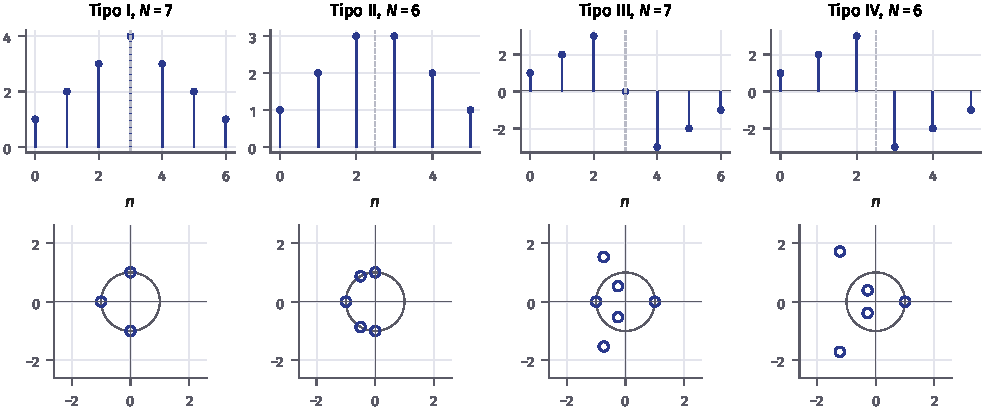
\includegraphics[width=\linewidth]{tipos_fase_lineal}
    \end{column}
  \end{columns}
  \herramienta{server/T4\_04\_FIR\_Fase\_Lineal.py}
\end{frame}

% =====================================================================
\section{Método de las ventanas}

\begin{frame}{Respuestas al impulso ideales}
  \small
  Con $h_d[n]=\frac{1}{2\pi}\int_{-\pi}^{\pi}H_d(\e^{j\Omega})\e^{j\Omega n}\dd\Omega$ y fase cero:
  \renewcommand{\arraystretch}{1.7}
  \begin{center}
    \begin{tabular}{@{}lll@{}}
      \toprule
      Filtro & $h_d[0]$ & $h_d[n]$, $n\ne0$\\\midrule
      Paso bajo ($\Omega_c$) & $\dfrac{\Omega_c}{\pi}$ & $\dfrac{\sin(\Omega_cn)}{\pi n}$\\
      Paso alto ($\Omega_c$) & $1-\dfrac{\Omega_c}{\pi}$ & $-\dfrac{\sin(\Omega_cn)}{\pi n}$\\
      Paso banda ($\Omega_1,\Omega_2$) & $\dfrac{\Omega_2-\Omega_1}{\pi}$ & $\dfrac{\sin(\Omega_2n)-\sin(\Omega_1n)}{\pi n}$\\
      Supresor ($\Omega_1,\Omega_2$) & $1-\dfrac{\Omega_2-\Omega_1}{\pi}$ & $-\dfrac{\sin(\Omega_2n)-\sin(\Omega_1n)}{\pi n}$\\\bottomrule
    \end{tabular}
  \end{center}
  \nota{El paso alto es $\delta[n]-h_{\text{PB}}[n]$ y el supresor $\delta[n]-h_{\text{BP}}[n]$. Un filtro multibanda es una suma de paso banda ponderados.}
\end{frame}

\begin{frame}{Truncar, ponderar y retrasar}
  \begin{center}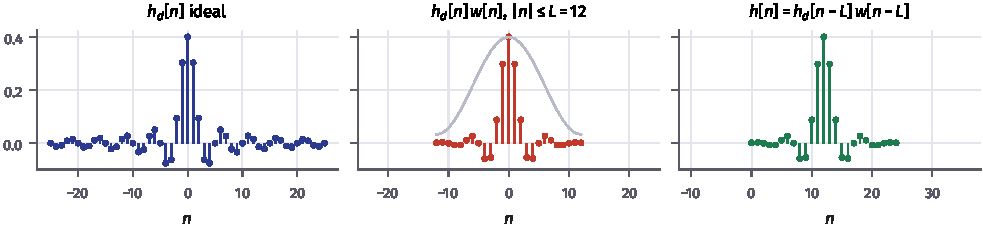
\includegraphics[width=\linewidth]{fir_ventana_metodo}\end{center}
  \begin{enumerate}\small
    \item Se trunca $h_d[n]$ a $\abs n\le L$ con una ventana: $h_w[n]=h_d[n]\,w[n]$, $N=2L+1$ coeficientes.
    \item Se retrasa $L$ muestras para hacerlo causal: $h[n]=h_w[n-L]$, $n=0,\dots,2L$.
  \end{enumerate}
  \begin{itemize}\small
    \item $h_d$ es par y $w$ también: $h$ es simétrica, \alert{tipo I}, con $H(\e^{j\Omega})=\e^{-j\Omega L}H_w(\e^{j\Omega})$ y $H_w$ real.
    \item Por el teorema de la modulación, $H_w=\frac1{2\pi}\,H_d\circledast W$: el ideal suavizado por la transformada de la ventana.
  \end{itemize}
\end{frame}

\begin{frame}{Truncamiento y fenómeno de Gibbs}
  \begin{center}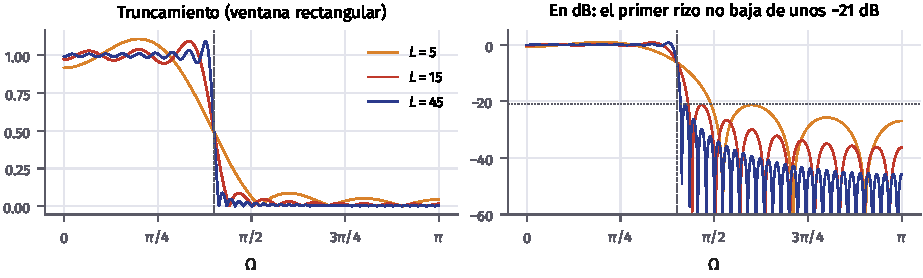
\includegraphics[width=0.92\linewidth]{gibbs}\end{center}
  \begin{itemize}\small
    \item El lóbulo principal de $W$ fija la \alert{anchura de la transición}: unos $4\pi/N$ con la ventana rectangular; se estrecha al crecer $L$.
    \item Los lóbulos secundarios fijan el \alert{rizado}: con la rectangular, un 9\,\% de sobreoscilación y unos $-21$\,dB en la banda de supresión, \alert{sea cual sea $L$} (Gibbs).
    \item Para bajar el rizado hay que cambiar de ventana, no alargarla.
  \end{itemize}
\end{frame}

\begin{frame}{Ventanas fijas}
  \begin{columns}[c]
    \begin{column}{0.44\textwidth}
      \small
      Para $-L\le n\le L$:
      \begin{align*}
        \text{Hann:}&\ \tfrac12+\tfrac12\cos\tfrac{2\pi n}{2L+1}\\
        \text{Hamming:}&\ 0{,}54+0{,}46\cos\tfrac{2\pi n}{2L+1}\\
        \text{Blackman:}&\ 0{,}42+0{,}5\cos\tfrac{2\pi n}{2L+1}\\&\ \ +0{,}08\cos\tfrac{4\pi n}{2L+1}
      \end{align*}
    \end{column}
    \begin{column}{0.54\textwidth}
      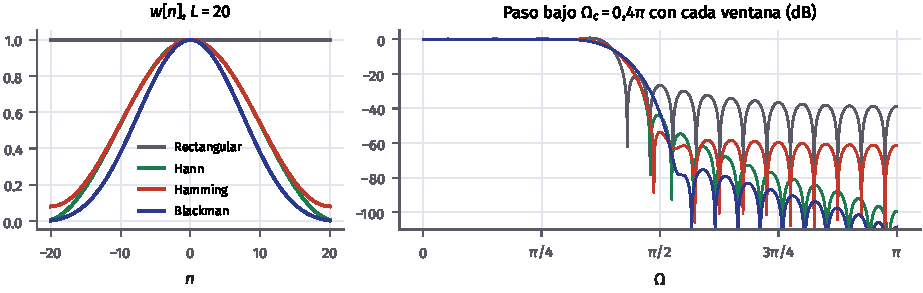
\includegraphics[width=\linewidth]{ventanas_fir}
    \end{column}
  \end{columns}
  \footnotesize
  \renewcommand{\arraystretch}{1.1}
  \begin{center}
    \begin{tabular}{@{}lcccc@{}}
      \toprule
      Ventana & Lóbulo principal & Lóbulo secundario & Atenuación mínima $\alpha_s$ & Transición $\Delta\Omega$\\\midrule
      Rectangular & $4\pi/(2L+1)$ & $-13{,}3$\,dB & 20,9\,dB & $0{,}92\pi/L$\\
      Hann & $8\pi/(2L+1)$ & $-31{,}5$\,dB & 43,9\,dB & $3{,}11\pi/L$\\
      Hamming & $8\pi/(2L+1)$ & $-42{,}7$\,dB & 54,5\,dB & $3{,}32\pi/L$\\
      Blackman & $12\pi/(2L+1)$ & $-58{,}1$\,dB & 75,3\,dB & $5{,}56\pi/L$\\\bottomrule
    \end{tabular}
  \end{center}
\end{frame}

\begin{frame}{Diseño con ventana fija}
  \begin{importante}[Receta]
    \begin{enumerate}
      \item Corte en el centro de la transición: $\Omega_c=(\Omega_p+\Omega_s)/2$, donde $\abs H\approx0{,}5$.
      \item La ventana más sencilla cuya atenuación mínima supere $\alpha_s$.
      \item $L$ tal que su transición sea menor que $\Delta\Omega=\Omega_s-\Omega_p$ (tabla).
    \end{enumerate}
  \end{importante}
  \begin{ejemplo}[$\Omega_p=0{,}3\pi$, $\Omega_s=0{,}5\pi$, $\alpha_s=40$\,dB]
    $\Omega_c=0{,}4\pi$, $\Delta\Omega=0{,}2\pi$. Sirven Hann, Hamming y Blackman:
    \[
      \text{Hann: }L\ge\frac{3{,}11\pi}{0{,}2\pi}=15{,}6\to16,\quad \text{Hamming: }L=17,\quad\text{Blackman: }L=28.
    \]
    La más corta es Hann: $N=33$ coeficientes y retardo de 16 muestras.
  \end{ejemplo}
  \nota{El rizado es el mismo en las dos bandas ($\delta_p\approx\delta_s$) y lo fija la ventana: con Hann, $\delta\approx0{,}0064$ (44\,dB).}
\end{frame}

\begin{frame}{En código: diseño con ventana de Hann}
  \codigo[basicstyle=\ttfamily\fontsize{6.8}{7.8}\selectfont]{fir_ventana}
  \nota{\texttt{hanning(N)} de Matlab no incluye los extremos nulos y \texttt{hann(N)} sí; \texttt{np.hanning(N)} los incluye, por eso se toma \texttt{np.hanning(N+2)[1:-1]}. \texttt{firwin} y \texttt{fir1} además normalizan la ganancia en $\Omega=0$.}
\end{frame}

\begin{frame}{Ventana de Kaiser}
  \begin{columns}[c]
    \begin{column}{0.5\textwidth}
      \small
      \[
        w[n]=\frac{I_0\big(\beta\sqrt{1-(n/L)^2}\big)}{I_0(\beta)},\quad \abs n\le L
      \]
      \begin{itemize}
        \item $I_0$: Bessel modificada de orden 0; $\beta$ ajusta el compromiso rizado–transición.
        \item Fórmulas empíricas de Kaiser:
      \end{itemize}
      \[
        \beta=\begin{cases}0{,}1102(\alpha_s-8{,}7)&\alpha_s>50\\0{,}5842(\alpha_s-21)^{0{,}4}\\\quad+0{,}07886(\alpha_s-21)&21\le\alpha_s\le50\\0&\alpha_s<21\end{cases}
      \]
      \[
        2L\ge\frac{\alpha_s-8}{2{,}285\,\Delta\Omega}
      \]
    \end{column}
    \begin{column}{0.48\textwidth}
      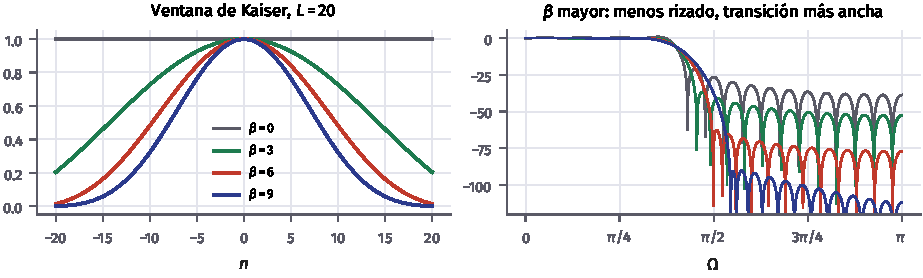
\includegraphics[width=\linewidth]{kaiser}
      \begin{ejemplo}[Mismas especificaciones]
        \footnotesize $\beta=0{,}5842\cdot19^{0,4}+0{,}07886\cdot19=3{,}395$; $2L\ge\frac{32}{2{,}285\cdot0{,}2\pi}=22{,}3\to L=12$: 25 coeficientes en lugar de 33.
      \end{ejemplo}
    \end{column}
  \end{columns}
  \herramienta{server/T4\_02\_FIR\_Kaiser.py}
\end{frame}

\begin{frame}{Comparación y otras ventanas ajustables}
  \begin{columns}[c]
    \begin{column}{0.5\textwidth}
      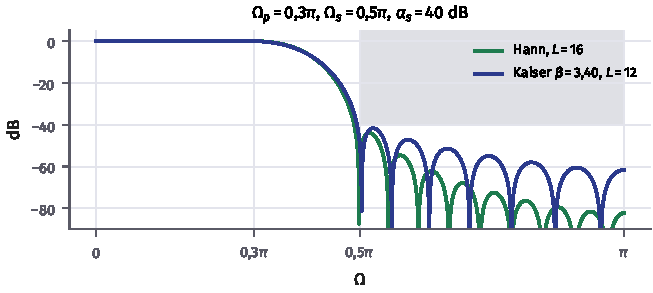
\includegraphics[width=\linewidth]{ejemplo_fir}
    \end{column}
    \begin{column}{0.48\textwidth}
      \small
      \begin{itemize}
        \item Las dos cumplen $\alpha_s=40$\,dB (44 y 41,7\,dB). Kaiser ajusta $\beta$ al requisito y no gasta coeficientes en exceso de atenuación.
        \item \alert{Dolph–Chebyshev} (\texttt{chebwin}): todos los lóbulos secundarios a la misma altura; $2L\approx\frac{2{,}056\alpha_s-16{,}4}{2{,}285\,\Delta\Omega}$.
        \item Si se dan rizados: $\alpha_s=-20\log_{10}\min(\delta_p,\delta_s)$, porque la ventana da el mismo en ambas bandas.
      \end{itemize}
    \end{column}
  \end{columns}
\end{frame}

\begin{frame}{En código: paso alto con Kaiser y con Parks–McClellan}
  \codigo{fir_kaiser}
  \nota{Un paso alto debe ser de tipo I ($N$ impar): un tipo II tendría un cero en $\Omega=\pi$.}
\end{frame}

% =====================================================================
\section{Otros métodos}

\begin{frame}{Diseño óptimo: Parks–McClellan}
  \begin{columns}[c]
    \begin{column}{0.5\textwidth}
      \footnotesize
      \begin{itemize}
        \item Minimiza el \alert{error máximo} ponderado entre $A(\Omega)$ y el ideal en las bandas especificadas (criterio minimax).
        \item La solución es \alert{equirrizada} (teorema de alternancia, algoritmo de Remez): con el mismo $N$, menos rizado que cualquier ventana.
        \item Estimación del orden (Kaiser):
        \[
          N-1\approx\frac{-20\log_{10}\sqrt{\delta_p\delta_s}-13}{14{,}6\,\Delta\Omega/2\pi}
        \]
        \item \texttt{firpm} (Matlab), \texttt{remez} (\texttt{scipy.signal}).
      \end{itemize}
    \end{column}
    \begin{column}{0.48\textwidth}
      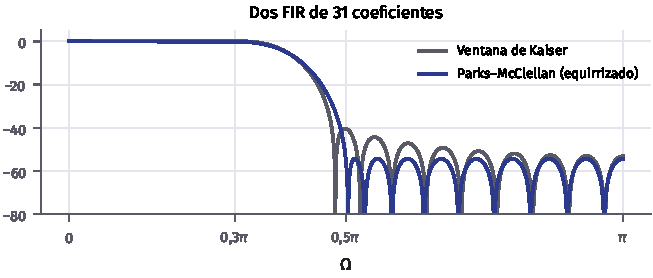
\includegraphics[width=\linewidth]{equirrizado}
    \end{column}
  \end{columns}
\end{frame}

\begin{frame}{Muestreo en frecuencia y filtros multibanda}
  \begin{columns}[c]
    \begin{column}{0.48\textwidth}
      \small
      \begin{itemize}
        \item Se fija la respuesta deseada en $N$ frecuencias $\Omega_k=2\pi k/N$ y se obtiene $h[n]$ con la IDFT (Tema 3), imponiendo simetría.
        \item Entre muestras la respuesta interpola, con rizado; se suaviza dejando muestras de transición o aplicando una ventana a $h[n]$.
        \item \texttt{fir2} (Matlab) y \texttt{firwin2} (\texttt{scipy.signal}) interpolan una respuesta definida a tramos, hacen la IDFT y aplican la ventana.
      \end{itemize}
    \end{column}
    \begin{column}{0.5\textwidth}
      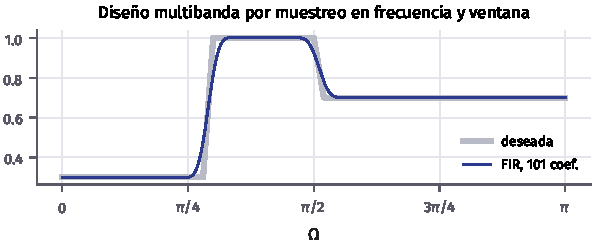
\includegraphics[width=\linewidth]{multibanda}
      \nota{\texttt{firwin2(101, [0,.28,.3,.5,.52,1], [.3,.3,1,1,.7,.7], window="hamming")}}
    \end{column}
  \end{columns}
\end{frame}

\begin{frame}{Coste y retardo}
  \small
  \begin{itemize}
    \item Un FIR de $N$ coeficientes cuesta $N$ productos por muestra (la mitad aprovechando la simetría) y retrasa $(N-1)/2$ muestras.
    \item Para órdenes de cientos o miles se filtra por bloques con la FFT (solapamiento y suma, Tema 3).
    \item Órdenes típicos en audio a 44,1--48\,kHz:
  \end{itemize}
  \footnotesize
  \begin{center}
    \begin{tabular}{@{}lll@{}}
      \toprule
      Aplicación & Coeficientes & Retardo aproximado\\\midrule
      Filtros básicos (ecualización, eliminación de ruido) & 50--200 & 1--2\,ms\\
      Filtros de cruce de altavoces & 100--500 & 1--5\,ms\\
      Cancelación de eco y reverberación & 500--2000 & 5--20\,ms\\
      Procesado de alta calidad (estaciones de audio digital) & 1000--5000 & 10--50\,ms\\\bottomrule
    \end{tabular}
  \end{center}
  \nota{En tiempo real el retardo limita el orden; un IIR o un FIR de fase mínima retrasan mucho menos.}
\end{frame}

% =====================================================================
\section*{Resumen}
\begin{frame}{Conceptos importantes}
  \begin{columns}[T]
    \begin{column}{0.5\textwidth}
      \begin{itemize}
        \item Simetría $h[n]=\pm h[N-1-n]$ $\Leftrightarrow$ fase lineal, retardo $(N-1)/2$.
        \item Cuatro tipos; los ceros forzados en $z=\pm1$ limitan qué filtros puede ser cada uno.
        \item Ventanas: truncar $h_d$, ponderar, retrasar $L$.
      \end{itemize}
    \end{column}
    \begin{column}{0.5\textwidth}
      \begin{itemize}
        \item La ventana fija el rizado; $L$, la transición.
        \item Kaiser: $\beta$ y $L$ por fórmula.
        \item Parks–McClellan: equirrizado, óptimo.
        \item Muestreo en frecuencia: respuestas arbitrarias.
      \end{itemize}
    \end{column}
  \end{columns}
  \bigskip
  \gris{Apuntes del Tema 4, sección 4 · Hoja de ejercicios, ejercicios 12–15.}
  \herramienta{server/T4\_01\_FIR\_Ventana\_Fija.py}
\end{frame}

\end{document}
